\section{Simulation experiments}
\begin{itemize}
	\item does num segments affect the initial ring velocity?
	\item does energy (and velocity) changes if Quantum=False?
	\item for a given R and euler method, what is the life of stability for various num segments
	\item when is it good to resegment?
	\item which config leads to the death of the ring for various R
	\item measure death time and distance for various R

\end{itemize}

\section{Vortex ring}
\begin{itemize}
	\item compare rings with various radii
	\item theoretical vs simulation velocity / range
	\item stability tests
	\item initialisation
	\item movement, decreasing radius
	\item comparison with theory
\end{itemize}

All presented measurements and results were done in purpose of setup the \texttt{config} file. We performed a tests with physical motivation and tests focused on precision and stability. With presented findings, there should be ensured the correctness and stability of any further high-scale simulation.

\subsection*{Frictionless test}

In case of zero temperature $T=0\unit{K}$, there should be no \textit{normal component} in superfluid He-II and therefore also no mutual friction. In such case, velocity and energy of vortex ring is conserved due to the lack of energy dissipation processes.

We plotted in \textbf{Figure 10} the ring velocity $\vert \vec{v}_c \vert $ and energy evoluting in time, for the case of $T=0$ and $T=1.5\unit{K}$. We tested the mutual friction effect during 1000 time-steps (\textit{epochs}) with varying $\text{d}t$.

\begin{figure}[h]
	\centering
	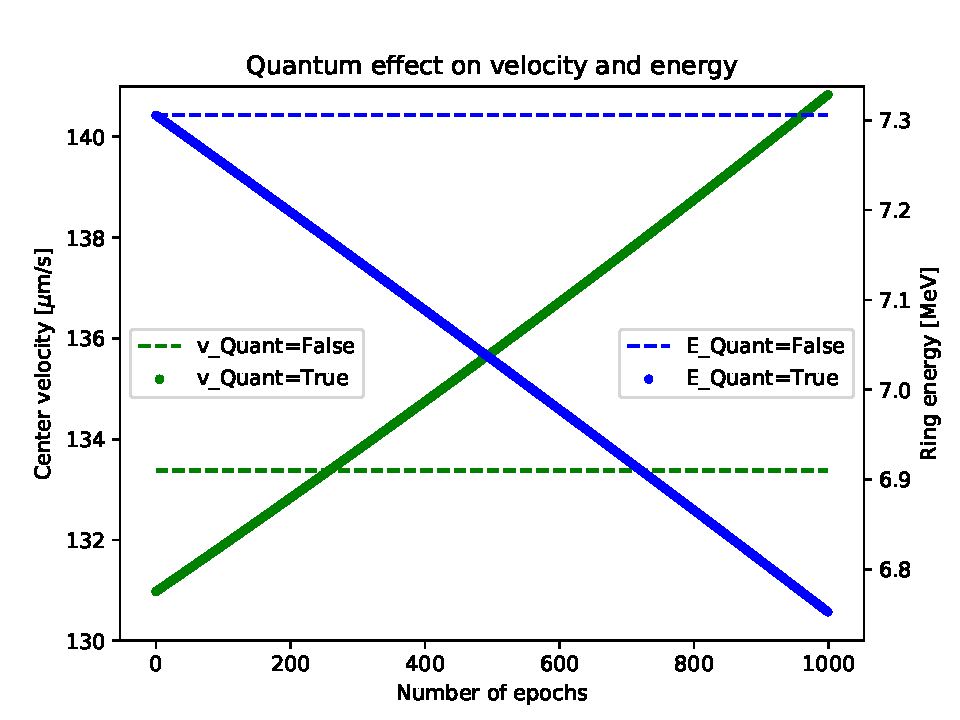
\includegraphics[width=0.8\textwidth]{graphics/results/Tzero}
	\caption{Dashed curves show the constant behaviour for temperature $T=0$), full lines the dissipation process for $T=1.5\text{K}$. On \texttt{x} axis, we plot the number of epochs (time steps) the vortex ring ran over and on \texttt{y} axis the velocity of ring center $\vert \vec{v}_c \vert $.}
\end{figure}

As we see, at $T=0\unit{K}$ the velocity and energy is conserved even after 1000 epochs of simulation. In case of $T>0$, energy is falling down as expected, whereas the velocity is increasing. This increase is physically well-explained by the fact that the radius is decreasing with time (\ref{ring-velocity}), also due to mutual friction.

\subsection*{Velocity precision test}

Our first velocity test compares the various approaches how can the ring velocity $\vert \vec{v}_c \vert $ be calculated. Here, we recognize between four approaches, based on its theoretical motivation, computational complexity and precision:
\begin{itemize}
	\item LIA (\ref{LIA}): motivated, cheap, not precise
	\item LIA + BIOT (\ref{LIA} + \ref{BIOT}): motivated, but expensive
	\item updated LIA (\ref{LIA_update}): not well motivated, but cheap and precise
	\item Theoretical (\ref{ring-velocity}): well motivated and precise
\end{itemize}
Of course, the theoretical velocity (\ref{ring-velocity}) is taken as a baseline that other velocites are compared with. All velocites were evoluted and measured during 5000 epochs (time steps), as we see in \textbf{Figure 11}.

\begin{figure}[h]
	\centering
	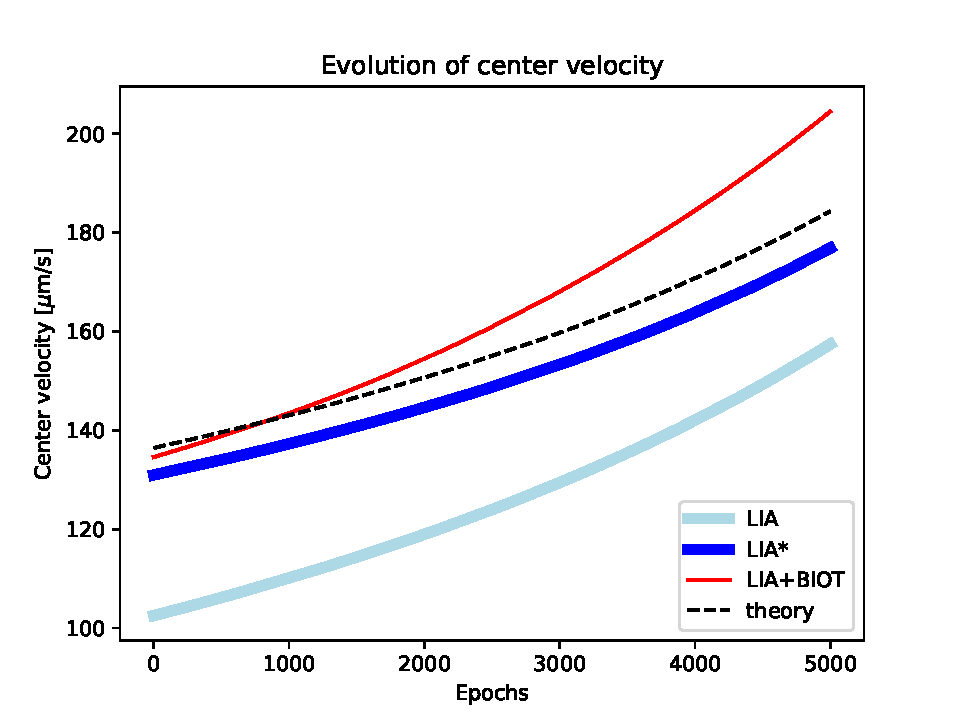
\includegraphics[width=0.8\textwidth]{graphics/results/vels_evolution}
	\caption{Comparison of all implemented velocity approaches (full lines) with the theoretical one (black dashed line). On \texttt{x} axis, we plot the number of epochs (time steps) the vortex ring ran over and on \texttt{y} axis the velocity of ring center $\vert \vec{v}_c \vert $.}
\end{figure}

As we see, the (LIA + BIOT) velocity grows much faster than it should according to theory. Therefore, for all further measurements we used the updated LIA velocity (LIA*) due to its precision and speed.

\subsection*{Velocity convergence test}

Next, we investigated the magnitude of ring velocity $\vert \vec{v}_c \vert $ for various resolutions $\delta \in \langle 50, 200 \rangle \mu\text{m}$, immediately after initialisation and then after 100 epochs. Ring radius was set at $R=1000\mu\text{m}$, so the number of discretisation points was given by $R$ and $\delta$ as $N \approx 2\pi R/ \delta \in \langle 30,120 \rangle$.

We see in \textbf{Figure 12} the expected convergent behaviour of both measured velocities in an area of good resolutions. Below $ \delta < 100 \mu\text{m}$, the velocites are enough convergent (corresponding to $\approx 60$ number of segments), which gives us the upper boundary.

\begin{figure}[h]
	\centering
	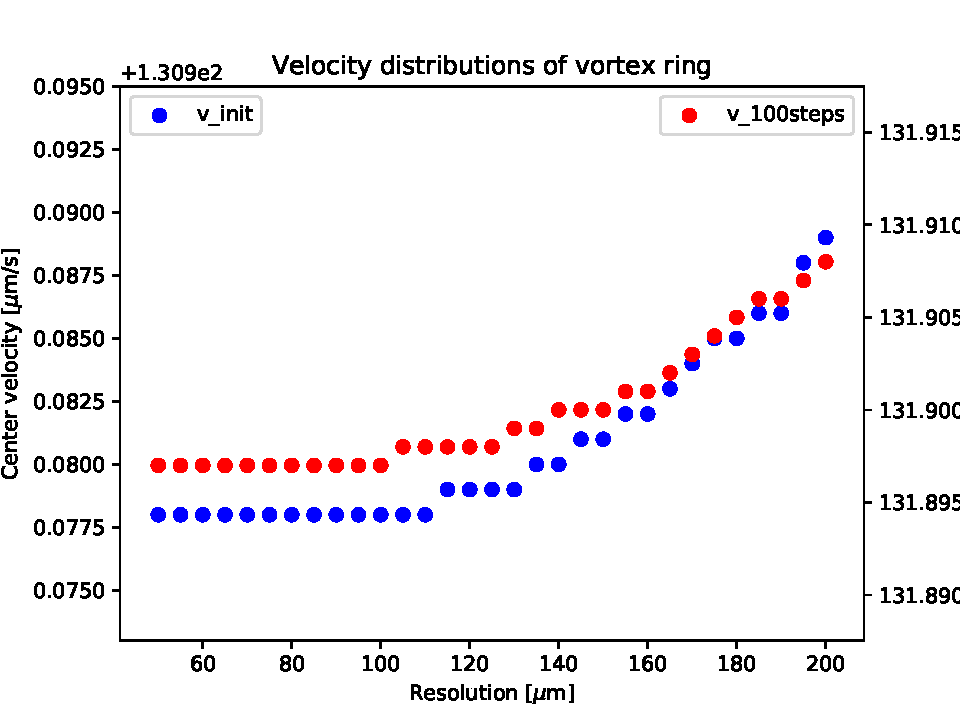
\includegraphics[width=0.8\textwidth]{graphics/results/vels_convergence}
	\caption{On \texttt{x} axis, we plot the resolutions $\delta$ and on \texttt{y} axis the velocity of ring center $\vert \vec{v}_c \vert $. Blue dots - initial ring velocities, Red dots - ring velocities after 100 epochs.}
\end{figure}

Even if it is intuitive that good resolutions lead to more stable velocities, the high number of vortex segments worsens the stability of simulation in time. Therefore, we propose also a lower boundary $\delta_{\text{min}}$, ensuring the stability, in a following test.

\subsection*{Stability test}

Stability of simulation was measured for three values of vortex radius $R \in \{500, 1000, 2000\} \mu\text{m}$ using \textit{Euler} and \textit{RK4} stepping in various resolutions. In all cases, the stability is described by the number of reached epochs, which was determined by the violation of length condition - the vortex circumference cannot deviate more than $1\%$ from the geometrical value $2\pi R$.

\newpage

\begin{figure}[h]
	\centering
	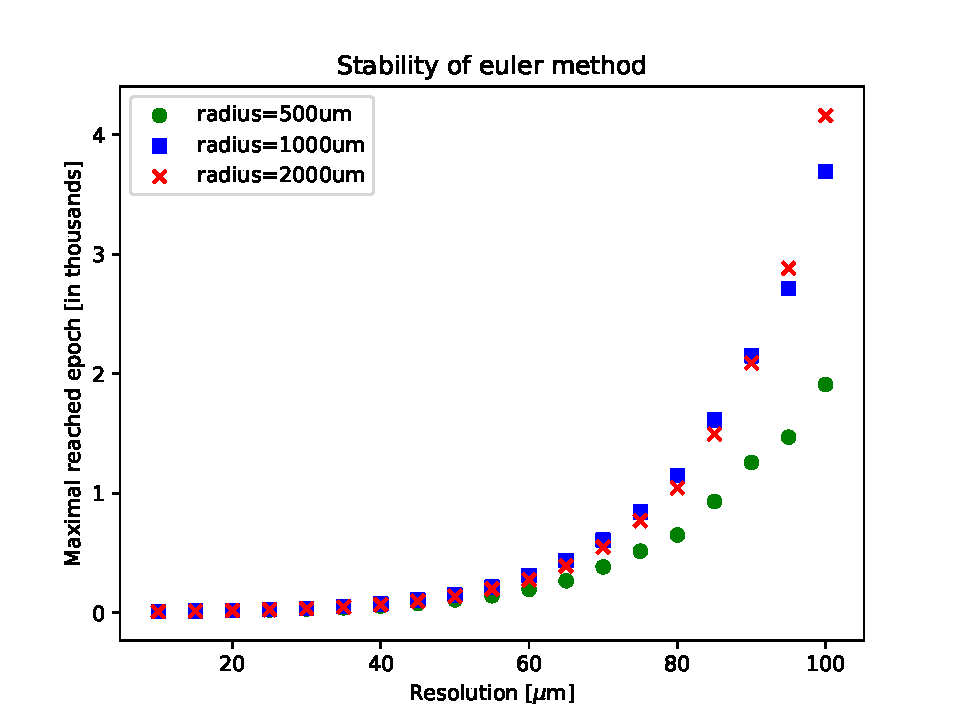
\includegraphics[width=0.8\textwidth]{graphics/results/stability-euler}
	\caption{Maximal reached epoch (time step) with Euler method till the simulation was killed by violating the length condition, for various radii $R$ and resolutions $\delta$.}
\end{figure}


Euler method seems to be instable for whatever resolution (\textbf{Figure 13}). Therefore it is useful only for test purposes. We recommend to use a way more stable method RK4 in a real high-scale simulation:

\begin{figure}[h]
	\centering
	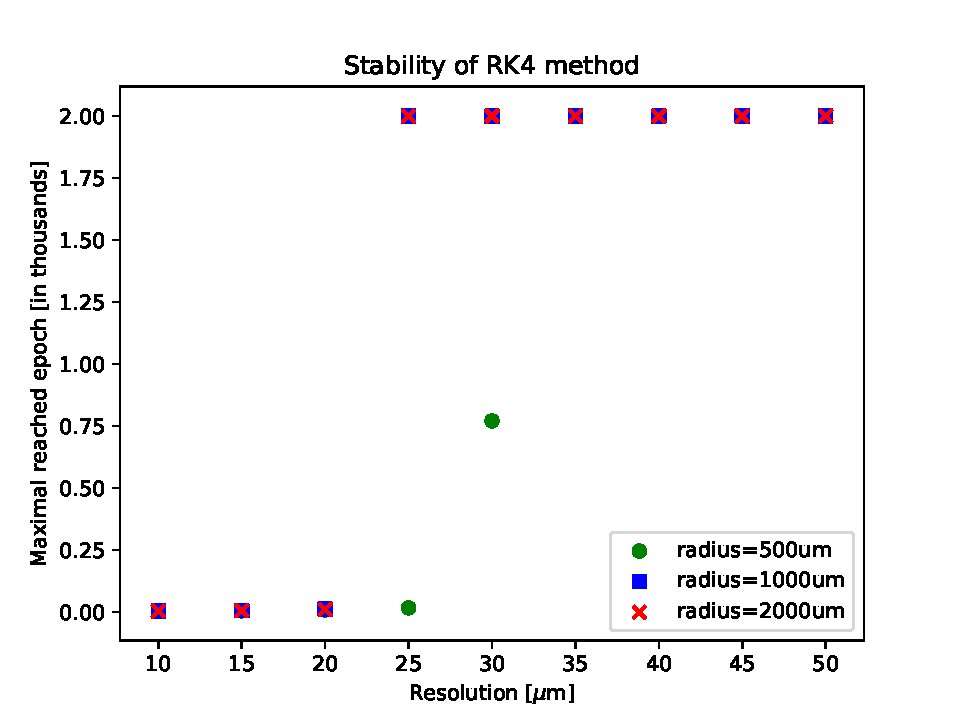
\includegraphics[width=0.8\textwidth]{graphics/results/stability-RK4}
	\caption{Maximal reached epoch (time step) with RK4 method till the simulation was killed by violating the length condition, for various radii $R$ and resolutions $\delta$. A threshold is set on $2000$ epochs.}
\end{figure}

The plot in \textbf{Figure 14} suggests the minimal resolution to be at least $\delta >30\mu\text{m}$. This boundary is still quite consevative, since the radius of vortex is decreasing in time (see Apendix part), so the resegmentation will happen. Resegmantation processes heavily help the simulation to be stable (deletes any forwarding numerical errors).

\newpage
